\section{PWM - Pulse Width Modulation}
\subsection{Introduzione}
E' un tipo di modulazione utilizzato largamente nell' elettronica di potenza.
In genere se si vuole comandare la tensione ai capi di un carico si deve ricorrere ad un circuito del genere:
\begin{figure}[H]
    \centering
    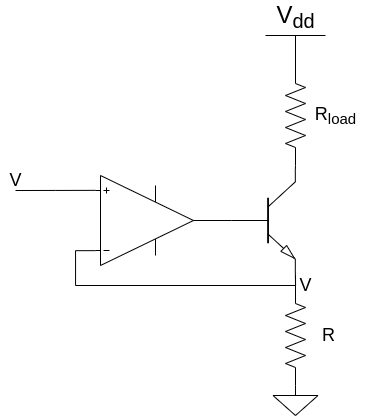
\includegraphics[width=150px]{images/19_PWM/power_dimmer.png}
\end{figure}
Quando si applica una tensione $V$ nell' ingresso non invertente dell' opamp per il cortocircuito virtuale ce l' abbiamo anche nell' ingresso invertente, quindi anche al capo della resistenza R.
Supponiamo di avere $V_{dd} = 12V$, $R = 1 \Omega$ e di applicare $V = 12V$ allora la potenza dissipata sulla resistenza $R$ è: $P = RI^2 = R \cdot \left( \frac{V}{R} \right)^2 = 144W$, se la tensione ai capi della resistenza è troppo grande possiamo abbassarla, supponiamo di variarla a $V = 6V$ la corrente che scorre in $R$ adesso è $I = \frac{V}{R} = 6A$ tuttavia ora molta potenza è dissipata anche sul transistor infatti abbiamo che $V_{CC} \cdot I_C = 36W$.

Se voglio evitare di dissipare potenza sul controllore (il transistor) devo passare ad un circuito con un transistore usato come interruttore:
\begin{figure}[H]
    \centering
    
\includegraphics[width=20px]{images/19_PWM/dimmer_with_switch.png}
\end{figure}
in questo modo quando chiudo il circuito ho una corrente di 12A, quando apro il circuito ho 0A, se volessi avere 6A potrei aprire per metà del tempo e chiudere per l' altra metà del tempo:
\begin{figure}[H]
    \centering
    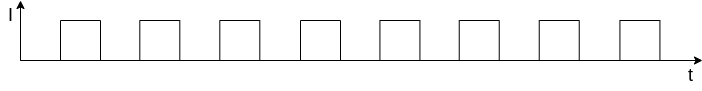
\includegraphics[width=320px]{images/19_PWM/duty_cycle.png}
\end{figure}
chiamiamo $t_{ON}$ il tempo in cui il circuito è chiuso e $t_{OFF}$ il tempo in cui il circuito è aperto allora definiamo:
$$ \delta = \frac{t_{ON}}{t_{ON} + t_{OFF}} = \text{duty cycle} $$

Uno degli inconvenienti di questo approcio è che il dispositivo alimentato non è effettivamente alimentato con una tensione intermedia ma acceso per un po' di tempo e spento per un altro po' di tempo, per alcuni carichi questo non è un problema (luci, led, motori, resistori per forni) per altri risulta essere problematico.

Calcoliamo la potenza lungo tutto il periodo: supponiamo che quando il transistor è chiuso si abbia potenza $P_0$ : 
$$ P = \frac{P_0 \cdot T_{ON} + 0 \cdot T_{OFF}}{T_{ON} + T_{OFF}} = P_0 \cdot \delta $$
la potenza sul carico è direttamente proporzionale a $\delta$ con $0 \leq \delta \leq 1$.
Si noti che questa è una potenza media in quanto calcolata su un intervallo.

La modulazione fatta in questo modo è semplice se eseguita da un microcontrollore, ovviamente si può fare senza logica con comparatori e maglie RC ma il circuito risulta più complesso.

Lo stesso segnale PWM generato posso usarlo per pilotare il controllore tradizionale, per fare ciò bisogna trasformare il segnale PWM in un segnale continuo, lo spettro dell' onda quadra generata è così composto:
\begin{figure}[H]
    \centering
    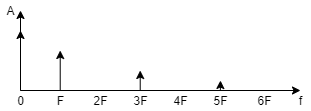
\includegraphics[width=200px]{images/19_PWM/pwm_spectre.png}
\end{figure}
abbiamo quindi le armoniche dispari ma anche una componente, il valore medio dell'onda, che è anche l'unica componente che ci interessa.

Per eliminare l' armonica fondamentale e tutte le altre successive usiamo un filtro passa basso che abbia frequenza di taglio minore della frequenza fondamentale: $F_H < F$, tipicamente $F_H = \frac{F}{10}$.
\begin{figure}[H]
    \centering
    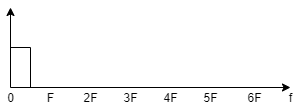
\includegraphics[width=200px]{images/19_PWM/ideal_filter.png}
\end{figure}
Ovviamente filtri del genere non esistono quindi ci affidiamo ad un filtro con un singolo polo che abbia una risposta in frequenza simile:
\begin{figure}[H]
    \centering
    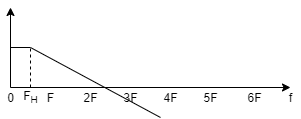
\includegraphics[width=200px]{images/19_PWM/actual_filter.png}
\end{figure}
Possiamo usare questo stesso valore continuo per pilotare il controllore analogico visto in precedenza.

Es: creiamo un dimmer led, comandiamo la corrente nel diodo luminoso, dato che la sua luce è proporzionale alla corrente possiamo scegliere l' intensità luminosa del LED.
$$ I = \frac{\delta \cdot V_{dd}}{R} $$
\begin{figure}[H]
    \centering
    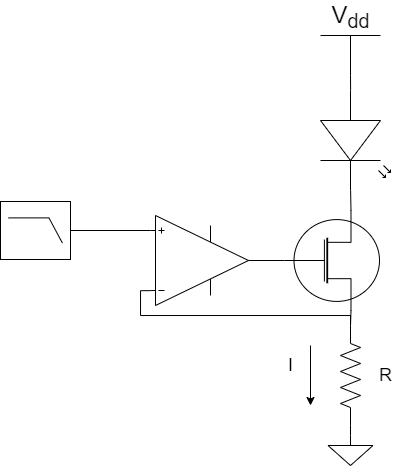
\includegraphics[width=200px]{images/19_PWM/pwm_led_dimmer.png}
\end{figure}

\subsection{Fast PWM}
Nel nostro microcontrollore il generatore PWM è costituito dal timer.
Preso un timer esso conta liberamente in avanti prima di tornare a 0:
\begin{figure}[H]
    \centering
    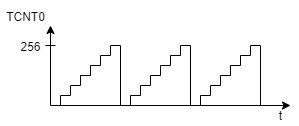
\includegraphics[width=200px]{images/19_PWM/fast_pwm_tcnt.png}
\end{figure}
in OCR ci mettiamo un valore ad 8 bit, quando il timer ha un valore minore di OCR in uscita poniamo 0, quando il valore in TCNT0 è maggiore di OCR mettiamo in uscita 1, oppure il contrario.
\begin{figure}[H]
    \centering
    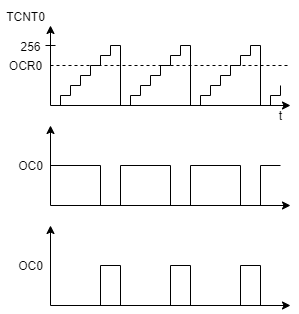
\includegraphics{images/19_PWM/non_inverting-inverting_fast_pwm.png}
\end{figure}
In alto modalità NON invertente, in basso modalità invertente.

All' aumentare di OCR0:
\begin{itemize}
    \item nella modalità NON invertente il $T_{ON}$ aumenta, quindi $\delta$ aumenta
    \item nella modalità invertente il $T_{ON}$ diminuisce, quindi $\delta$ diminuisce
\end{itemize}

Dato che i valori sono interi non possiamo avere tutti i valori possibili di $\delta$, la risoluzione del periodo è $\Delta\delta = \frac{1}{256} = 0.4\%$.

Il periodo di questo PWM è $T = 256 \cdot t_{CK} \cdot P$ in cui $t_{CK}$ è il periodo del clock mentre $P$ è il valore corrente del prescaler, quindi 1, 8, 64, 256 o 1024.

La frequenza massima si ha per $t_{CK}$ minima e $P=1$, usando il timer0 con clock di 1MHz $t_{CK} = 1 \mu s$ quindi il periodo è di $256 \mu s$ quindi la frequenza è $f = \frac{1}{256\mu s} = 4KHz$.
Volendo uscire dalla banda audio si deve andare oltre i 20KHz, usando clock a 4MHz la frequenza è già $f = 16KHz$ che è ai limiti della banda audio, solitamente udibile da ben poche persone, quindi va già bene.

Usando il timer1 non si ha un conteggio a 16 bit, se lo facesse si avrebbe una frequenza PWM bassissima, ad esempio con clock a 1MHz la frequenza sarebbe $f = \frac{1}{256^2 \mu s} = 15Hz$, per evitare ciò si è pensato di dotare il timer1 di 3 modalità PWM che permettono di avere risoluzioni a:
\begin{itemize}
    \item 8 bit: 0-255
    \item 9 bit: 0-511
    \item 10 bit: 0-1023
\end{itemize}
Es: a 10 bit $\Delta \delta = 0.001$ ma la frequenza diminuisce in quanto il periodo aumenta di 4 volte.

Nella maggior parte dei casi l' importante è avere una frequenza alta e non una risoluzione alta.

Abbiamo in totale 4 generatori PWM indipendenti:
\begin{itemize}
    \item timer 0 ha 1 generatore PWM ad 8 bit
    \item timer 1 ha 2 PWM con OCRA ed OCRB
    \item timer 2 ha 1 generatore PWM identico a quello di timer 0
\end{itemize}

\begin{figure}[H]
    \centering
    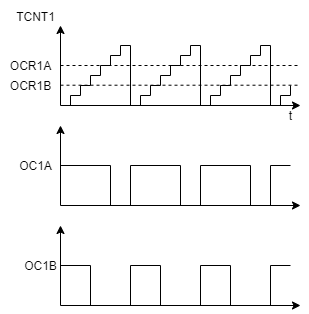
\includegraphics[width=200px]{images/19_PWM/pwm_timer_1.png}
\end{figure}

\subsection{PWM a fase corretta}
Essendo un segnale rettangolare il baricentro degli impulsi si trova nel centro del rettangolo.
Facendo la trasformata di Fourier del segnale la componente sinusoidale fondamentale ha questa forma:
\begin{figure}[H]
    \centering
    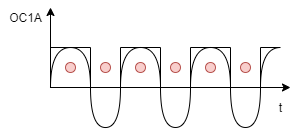
\includegraphics[width=200px]{images/19_PWM/pwm_center_of_gravity.png}
\end{figure}
Il massimo della sinusoide è nel baricentro del $T_{ON}$, il minimo è nel baricentro del $T_{OFF}$, che sono spaziati di un semiperiodo.
Se vario OCRA il margine destro dell' impulso si sposta e con lui anche il baricentro, quindi la sinusoide: cambiano le fasi delle armoniche che costituiscono il segnale.

In certe applicazioni la fase del segnale è importante, ad esempio se abbiamo due motori che sono alimentati da due segnali diversi alla stessa frequenza in base alla fase di ogni segnale abbiamo che i disturbi dei due motori possono sommarsi oppure cancellarsi l' uno con l' altro.

Se non si vogliono avere problemi di sorta con la fase del segnale anziché usare il fast PWM possiamo passare al PWM a fase corretta.

In questa modalità il contatore conta up-down, cioè prima conta da 0 a 255 e poi da 255 a 0:
\begin{figure}[H]
    \centering
    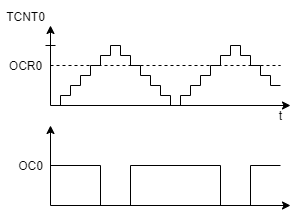
\includegraphics[width=200px]{images/19_PWM/phase_correct_pwm.png}
\end{figure}
in questa modalità se cambio OCR a spostarsi sono entrambi i lati del rettangolo $T_{ON}$ quindi il baricentro rimane fermo.
Tuttavia il periodo questa volta è raddoppiato in quanto dobbiamo contare il doppio:
$$ T = 2 \cdot 256 \cdot t_{CK} \cdot P $$

\subsection{Glitch}
Se cambio la configurazione del timer mentre è in corso potrebbe accadere che in alcuni periodi si abbiano due $T_{ON}$, per evitare ciò si consiglia di aggiornare i registri quando il contatore è al massimo o al minimo.

\subsection{Configurazione nel uC}
\subsubsection{Timer 0}
Per configurare quale modalità PWM si usano i bit WGM:
\begin{table}[H]
    \centering
    \begin{tabular}{c c | l}
        WGM01 & WGM00 & Descrizione \\
        \hline
        0 & 1 & PWM a fase corretta \\
        \hline
        1 & 1 & Fast PWM \\
        \hline
    \end{tabular}
\end{table}
Per configurare l' inversione del PWM si usano i bit COM00 e COM01:
\begin{table}[H]
    \centering
    \begin{tabular}{c c | l}
        COM01 & COM00 & Descrizione \\
        \hline
        0 & 0 & OC0 disconnesso \\
        \hline
        0 & 1 & - \\
        \hline
        1 & 0 & NON invertente \\
        \hline
        1 & 1 & invertente \\
        \hline
    \end{tabular}
\end{table}
il clock si sceglie sempre tramite i bit CS.

\subsubsection{Timer 1}
Per il timer 1 valgono le stesse considerazioni ma abbiamo molte più configurazioni del PWM perché possiamo usarlo a 8, 9, 10 bit.

\subsubsection{Timer 2}
Il timer 2 è identico al timer 1 con l' aggiunta della possibilità di usare una sorgente esterna come clock del timer.

